% Figures/minimization_plot.tex
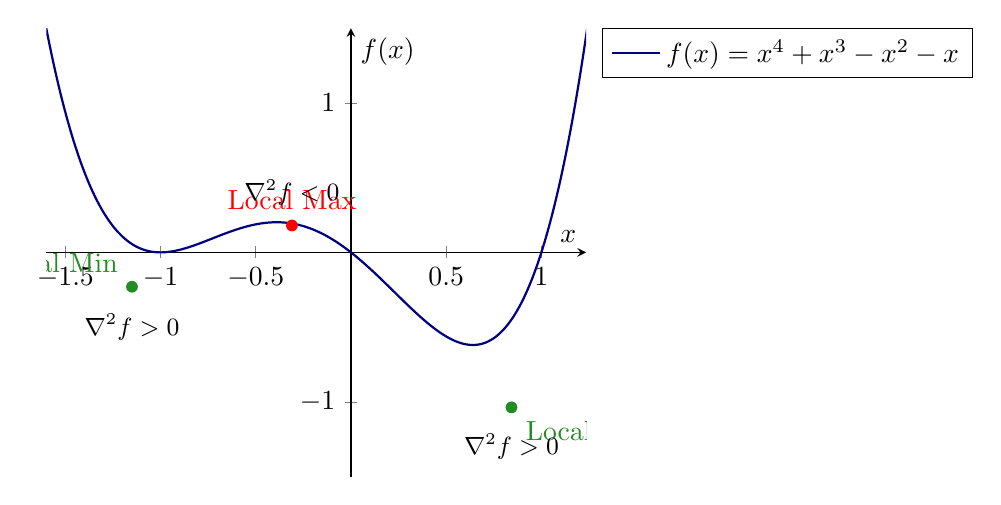
\begin{tikzpicture}
    \begin{axis}[
        axis lines=middle,
        xlabel=$x$,
        ylabel={$f(x)$},
        samples=200,
        domain=-1.75:1.25,
        ymin=-1.5,
        ymax=1.5,
        legend pos=outer north east,
        ]
        \addplot[thick, NavyBlue, smooth] {x^4 + x^3 - x^2 - x};
        \addlegendentry{$f(x) = x^4 + x^3 - x^2 - x$}

        % Minima and Maxima
        \node[circle, fill=ForestGreen, inner sep=1.5pt, label={[ForestGreen]below right:Local Min}] at (axis cs:0.843, -1.037) {};
        \node[circle, fill=ForestGreen, inner sep=1.5pt, label={[ForestGreen]above left:Local Min}] at (axis cs:-1.15, -0.23) {};
        \node[circle, fill=Red, inner sep=1.5pt, label={[Red]above:Local Max}] at (axis cs:-0.31, 0.18) {};

        % Hessian signs
        \node[font=\small] at (axis cs:0.843, -1.3) {$\nabla^2 f > 0$};
        \node[font=\small] at (axis cs:-1.15, -0.5) {$\nabla^2 f > 0$};
        \node[font=\small] at (axis cs:-0.31, 0.4) {$\nabla^2 f < 0$};
    \end{axis}
\end{tikzpicture}
